\documentclass[ucs,9pt,pagenumbersfull]{beamer}

\usetheme{gray}

%% To create high resolution - for print outs
%\usepackage{pgfpages}
%\pgfpagesuselayout{resize to}[a4paper,border shrink=5mm,landscape]
%\mode<handout>{\setbeamercolor{background canvas}{bg=black!5}}

\def\vRad{2pt} % Radius of vertices in TikZ images

\setbeameroption{show notes}

\logosmall{logos/fu_small_logo}
\logobig{logos/fu_big_logo}
\logoaux{logos/cglLogo}
\logoauxx[1.cm]{logos/bms-logo-with-text}
\titleimage[2.92cm]{Figures/Title_picture}

\title[Contact Surfaces Parameterization] % (optional, use only with long paper titles)
{On the Parameterization and the \mbox{Geometry} of the \mbox{Configuration} Space of a Single \mbox{Planar} Robot}
% Optional subtitle
%\subtitle{Optional subtitle}

\author[Atariah,~Rote] % (optional, use only with lots of authors)
{Dror Atariah \and Günter Rote}
% - Give the names in the same order as the appear in the paper.

\institute[FU Berlin] % (optional, but mostly needed)
{Freie Universität Berlin}

\date[WSCG'13] % (optional, should be abbreviation of conference name)
{June 27\textsuperscript{th} 2013}
% - Either use conference name or its abbreviation.
% - Not really informative to the audience, more for people (including
%   yourself) who are reading the slides online

% Delete this, if you do not want the table of contents to pop up at
% the beginning of each subsection:
\AtBeginSection[]
{
  \begin{frame}<beamer>{Outline}
    \tableofcontents[currentsection]
  \end{frame}
}
\AtBeginSubsection[]
{
  \begin{frame}<beamer>{Outline}
    \tableofcontents[currentsubsection]
  \end{frame}
}

\begin{document}

\begin{frame}[plain]
  \titlepage
\end{frame}

\begin{frame}{Outline}
  \tableofcontents
  % You might wish to add the option [pausesections]
\end{frame}

\section{Introduction}

\begin{frame}
  \frametitle{Setting}
  \begin{minipage}{.4\linewidth}
    \begin{overlayarea}{\textwidth}{0.6\textheight}
      \only<1-2>{
        A planar polygonal (convex) robot \(\mathcal{A}\) moving amid
        polygonal (convex) obstacles \(\{ \mathcal{O}_j \}_{j\in
          J}\).

        \begin{block}{Free\dots}
          Can be either in a \emph{free configuration}
          \(\mathcal{C}_{free}\).
        \end{block}

      }
      \only<2>{
        \begin{block}{Forbidden\dots}
          \emph{Or,} forbidden one \(\mathcal{C}_{forb} = \mathcal{C}
          \setminus \mathcal{C}_{free} \).
        \end{block}

      }
    \end{overlayarea}
  \end{minipage}
  \hfill
  \begin{minipage}{.55\linewidth}
    \begin{overlayarea}{\textwidth}{\textheight}
      \begin{figure}
        \centering
        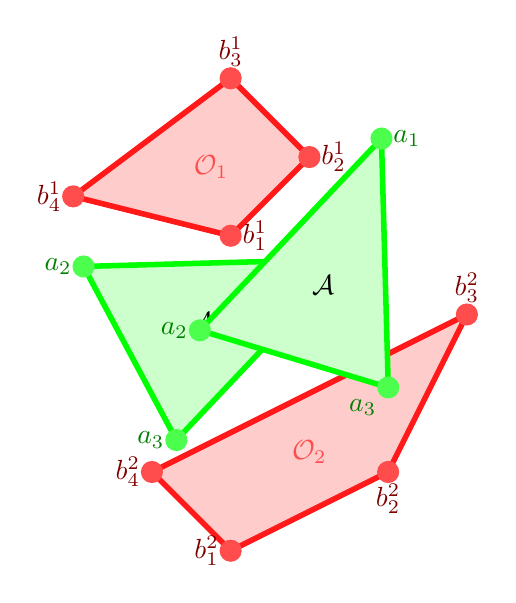
\begin{tikzpicture}[%
  obstacle/.style={line join=round,red!90,fill=red!20,line width=\vRad},
  obstacle vertices/.style={red!70},
  obstacle vertices label/.style={red!50!black},
  robot/.style={line join=round,green,fill=green!20,line width=\vRad},
  robot vertices/.style={green!70},
  robot vertices label/.style={green!50!black}
  ]

  \coordinate (b11) at (3,4);
  \coordinate (b12) at (4,5);
  \coordinate (b13) at (3,6);
  \coordinate (b14) at (1,4.5);

  \draw[obstacle] %
  (b11)node[obstacle vertices label,right]{$b_1^1$} --
  (b12)node[obstacle vertices label,right]{$b_2^1$} --
  (b13)node[obstacle vertices label,above]{$b_3^1$} --
  (b14)node[obstacle vertices label,left]{$b_4^1$} -- cycle;
  \foreach \i in {1,2,3,4}
  \fill[obstacle vertices] (b1\i) circle (2*\vRad);
  \node[obstacle vertices] at (barycentric cs:b11=0.25,b12=0.25,b13=0.25,b14=0.25) {$\mathcal{O}_1$};

  \coordinate (b21) at (3,0);
  \coordinate (b22) at (5,1);
  \coordinate (b23) at (6,3);
  \coordinate (b24) at (2,1);

  \draw[obstacle] %
  (b21)node[obstacle vertices label,left]{$b_1^2$} --
  (b22)node[obstacle vertices label,below]{$b_2^2$} --
  (b23)node[obstacle vertices label,above]{$b_3^2$} --
  (b24)node[obstacle vertices label,left]{$b_4^2$} -- cycle;
  \foreach \i in {1,2,3,4}
  \fill[obstacle vertices] (b2\i) circle (2*\vRad);
  \node[obstacle vertices] at (barycentric cs:b21=0.25,b22=0.25,b23=0.25,b24=0.25) {$\mathcal{O}_2$};

  \onslide<1>{
    \begin{scope}[rotate=-25,xshift=-2.5cm,yshift=0.25cm]
      \coordinate (a1) at (5,5);%
      \coordinate (a2) at (2,3.5);%
      \coordinate (a3) at (4,2);%
      \draw[robot] %
      (a1)node[robot vertices label,right]{$a_1$} --
      (a2)node[robot vertices label,left]{$a_2$} --
      (a3)node[robot vertices label,left]{$a_3$} -- cycle;%
      \foreach \i in {1,2,3}%
      \fill[robot vertices] (a\i) circle (2*\vRad);%
      \node at (barycentric cs:a1=0.3333,a2=0.33333,a3=0.3333) {$\mathcal{A}$};
    \end{scope}
  }

  \onslide<2>{
    \begin{scope}[xshift=0.75cm,yshift=-0.5cm,rotate around={20:(2.5,3)}]
      \coordinate (a1) at (5,5);%
      \coordinate (a2) at (2,3.5);%
      \coordinate (a3) at (4,2);%
      \draw[robot] %
      (a1)node[robot vertices label,right]{$a_1$} --
      (a2)node[robot vertices label,left]{$a_2$} --
      (a3)node[robot vertices label,below left]{$a_3$} -- cycle;%
      \foreach \i in {1,2,3}%
      \fill[robot vertices] (a\i) circle (2*\vRad);%
      \node at (barycentric cs:a1=0.3333,a2=0.33333,a3=0.3333) {$\mathcal{A}$};
    \end{scope}
  }
\end{tikzpicture}
%%% Local Variables:
%%% mode: latex
%%% TeX-master: "../main"
%%% End:

      \end{figure}
    \end{overlayarea}
  \end{minipage}
\end{frame} %Setting

\begin{frame}
  \frametitle{Contact Types}
  \begin{minipage}{0.4\linewidth}
    \begin{overlayarea}{\textwidth}{0.6\textheight}
      \only<1->{
        We consider two \emph{main} types of contacts:
        \begin{itemize}
        \item Vertex-Edge
        \item Edge-Vertex
        \end{itemize}
      }

      \only<2->{
        We can have two additional types of contact:
        \begin{itemize}
        \item Vertex-Vertex
        \item Edge-Edge
        \end{itemize}
      }
    \end{overlayarea}
  \end{minipage}
\note<2->{
  First type of contacts have 2 DOF

  Second type of contacts have \emph{only} 1 DOF
}
  %
  \hfill
  \begin{minipage}{0.55\linewidth}
    \begin{center}
      \begin{tikzpicture}
  \tikzset{x=10pt,y=10pt}
  % Robot's vertices definition
  \coordinate (a1) at (5,0);
  \coordinate (a2) at (1,4);
  \coordinate (a3) at (-3.5,-1.0);
  \coordinate (a4) at (0,-3);
  \node[green,right=0.5em] at (a1){$a_1$};
  \node[green,right=0.5em] (ve) at (a2){$a_2$};
  \node[green,left=0.5em] at (a3){$a_3$};
  \node[green,below=0.5em] at (a4){$a_4$};

  % Robot's polygon
  \draw[line join=round,green,fill=green!20,line width=\vRad] (a1) -- node[right]
  {$e_{1,2}$} (a2) -- node[left] {$e_{2,3}$} (a3) -- node[below=0.2em]
  {$e_{3,4}$} (a4) -- node[below=0.2em] {$e_{4,1}$} (a1) -- cycle;
  \node[green] at (barycentric cs:a1=0.25,a2=0.25 ,a3=0.25,a4=0.25){$\mathcal{A}$};
  % Robot's vertices plotting
  \foreach \pts in {a1,a2,a3,a4}
  \fill [green!70] (\pts) circle (2*\vRad);

  \def\oAngle{101}
  % Defining the vertices relative to (a2), and making sure it
  % is tangent.
  \coordinate (a2tmp) at ($(a2)+(\oAngle:2.5*\vRad)$);
  \coordinate (b11) at ($(a2tmp)+(\oAngle+90:3)$); \coordinate
  (b21) at ($(a2tmp)+(\oAngle-90:2)$); \coordinate (b31) at
  ($(a2tmp)+(\oAngle+5:4.5)$); \node [red,left=0.2em] at (b11)
  {$b_1^1$}; \node [red,right=0.2em] at (b21) {$b_2^1$}; \node
  [red,above=0.2em] at (b31) {$b_3^1$};

  % 1st obstacle's polygon
  \draw[line join=round,red!90,fill=red!20,line width=\vRad]
  (b11) -- (b21) -- (b31) -- cycle; \node[red] at (barycentric
  cs:b11=0.333,b21=0.333,b31=0.333){$\mathcal{O}_1$};

  \foreach \pts in {b11,b21,b31} \fill [red!70] (\pts) circle
  (2*\vRad);

  %%%%%
  % 2nd obstacle
  \coordinate (b12tmp) at ($(a4)!(10,-11)!(a1)$); \coordinate
  (b12) at ($(b12tmp)!2.5*\vRad!(10,-11)$); \node[above right]
  (ev) at (b12){}; \coordinate (b22) at ($(b12)+(355:5)$);
  \coordinate (b32) at ($(b12)+(290:5.2)$);

  \draw[line join=round,red!90,fill=red!20,line width=\vRad]
  (b12) -- (b22) -- (b32) -- cycle; \node[red] at (barycentric
  cs:b12=0.333,b22=0.333,b32=0.333){$\mathcal{O}_2$};

  \foreach \pts in {b12,b22,b32} \fill [red!70] (\pts) circle
  (2*\vRad);

  %%%%%%
  % Annotating
  \draw[blue,<-,line width=0.25*\vRad] (ve) .. controls
  ($(ve)+(-15:3.5)$) .. ($(ve)+(5,6)$);
  \node[blue,above,align=center] at ($(ve)+(5,6)$)
  {Vertex-Edge\\Contact};

  \draw[blue,<-,line width=0.25*\vRad] (ev) .. controls
  ($(ev)+(5:5)$) .. ($(ev)+(5,4)$);
  \node[blue,above,align=center] at ($(ev)+(5,4)$)
  {Edge-Vertex\\Contact};
\end{tikzpicture}
%%% Local Variables:
%%% mode: latex
%%% TeX-master: "../main"
%%% End:

    \end{center}
  \end{minipage}
\end{frame}

\begin{frame}
  \frametitle{General Problem Statement}
  \begin{block}{Ultimate Goal}
    Find a \emph{collision free} path for \(\mathcal{A}\) to move from a start point to a
    target point.
  \end{block}

  \begin{figure}
    \centering
    \begin{tikzpicture}
  \tikzset{x=9pt,y=9pt}
  %%%%
  % Robot
\newcommand{\plotRobot}{
  \begin{scope}%[rotate=\ortAngle]
    \coordinate (a1) at ($(\Rx,\Ry)+(0+\ortAngle:2)$);
    \coordinate (a2) at ($(\Rx,\Ry)+(100+\ortAngle:4)$);
    \coordinate (a3) at ($(\Rx,\Ry)+(276+\ortAngle:1)$);

    \draw [line join=round,green,fill=green!20, line width =\vRad,opacity=0.8] (a1)  -- (a2) -- (a3) -- cycle;

    \foreach \pts in {a1,a2,a3}
    \fill [green!70] (\pts) circle (2*\vRad);
  \end{scope}
}
\draw[step=1,black!20] (-15,-8) grid (15,8);
\coordinate (b11) at (1,1);
\coordinate (b21) at (1,4);
\coordinate (b31) at (-1,3);
\coordinate (b41) at (-1,-1);
\draw[line join=round,red!90,fill=red!20,line width=\vRad,opacity=0.7] (b11) -- (b21) -- (b31)  -- (b41) -- cycle;
\foreach \pts in {b11,b21,b31,b41}
\fill [red!70] (\pts) circle (2*\vRad);

\coordinate (b12) at (-5,-3);
\coordinate (b22) at (-8,-1);
\coordinate (b32) at (-6,-6);
\coordinate (b42) at (-4,-4);
\draw[line join=round,red!90,fill=red!20,line width=\vRad,opacity=0.7] (b12) -- (b22) -- (b32)  -- (b42) -- cycle;
\foreach \pts in {b12,b22,b32,b42}
\fill [red!70] (\pts) circle (2*\vRad);

\coordinate (b13) at (10,1);
\coordinate (b23) at (7,4);
\coordinate (b33) at (6,-3);
\draw[line join=round,red!90,fill=red!20,line width=\vRad,opacity=0.7] (b13) -- (b23) -- (b33) -- cycle;
\foreach \pts in {b13,b23,b33}
\fill [red!70] (\pts) circle (2*\vRad);

\draw[->,dashed,blue,line width=\vRad] (-10,4) .. controls +(-10:5) .. (-2.5,-3.5) .. controls +(-40:5) and (270:2) .. (4,2) .. controls +(100:5) and (30:15) .. (10,4);


\newcommand{\Rx}{-10}
\newcommand{\Ry}{4}
\newcommand{\ortAngle}{20}
\plotRobot{}

\renewcommand{\Rx}{-2.5}
\renewcommand{\Ry}{-3.5}
\renewcommand{\ortAngle}{40}
\plotRobot{}

\renewcommand{\Rx}{4}
\renewcommand{\Ry}{2}
\renewcommand{\ortAngle}{-20}
\plotRobot{}

\renewcommand{\Rx}{10}
\renewcommand{\Ry}{4}
\renewcommand{\ortAngle}{-90}
\plotRobot{}

\end{tikzpicture}
%%% Local Variables:
%%% mode: latex
%%% TeX-master: "../main"
%%% End:

  \end{figure}
\end{frame}

\section{Configuration Space}
\begin{frame}
  \frametitle{The Configuration Space}
  A robot's configuration (pose) is determined by a \emph{translation vector} \(\vec{r}=(x,y) \in \mathbb{R}^2\) and an \emph{orientation angle} \(\theta\in S^1\).

  \begin{definition}[Configuration Space]
    The space \(\mathcal{C} = \left( \mathbb{R}^2 \times S^1 \right)\) is called the \emph{configuration space} of a given robot \(\mathcal{A}\).

    \begin{itemize}
    \item \(\mathcal{C}_{free} = \left\{ q \in \mathcal{C} \mid \,
        \mathcal{A}(q) \cap \left(\bigcup_{j} \mathcal{O}_j\right)=
        \emptyset \right\} \)
    \item \(\mathcal{C}_{forb}  = \mathcal{C} \setminus \mathcal{C}_{free}\)
    \end{itemize}
  \end{definition}
\end{frame}

\begin{frame}
  \frametitle{From \(\mathcal{C}\)-space to the real world}
  Given a point \(q=\left(x,y,\theta\right)\in \mathcal{C}\), the
  corresponding configuration of the robot in the \emph{work space} is given by:
  \[
  a_i(q) = \binom{x}{y}+r_i \binom{\cos(\alpha_i + \theta)}{\sin(\alpha_i+\theta)}
  \]

  \begin{figure}
    \centering
    \begin{tikzpicture}
  \tikzset{x=7pt,y=7pt}

  \newcommand{\plotRobot}{
      \coordinate (a1) at ($(\Rx,\Ry)+(-30+\ortAngle:6)$);
      \coordinate (a2) at ($(\Rx,\Ry)+(110+\ortAngle:8)$);
      \coordinate (a3) at ($(\Rx,\Ry)+(250+\ortAngle:4)$);

      \draw [line join=round,green,fill=green!20, line width =\vRad,opacity=0.8] (a1)  -- (a2) -- (a3) -- cycle;

      \foreach \pts in {a1,a2,a3}
      \fill [green!70] (\pts) circle (2*\vRad);
  }

  \def\Rx{0}
  \def\Ry{0}
  \def\ortAngle{0}
  \def\tX{-15}
  \def\tY{10}

\onslide<3>{
  \def\rotAngle{0}
  \begin{scope}[shift={(\tX,\tY)},rotate=\rotAngle]
    \plotRobot{}
    \coordinate (R0) at (\Rx,\Ry);
    \fill[green] (R0) circle (\vRad);
    \draw[gray,->] (R0) -- ($(R0)+(2,0)$);
    \draw[gray,->] (R0) -- ($(R0)+(0,2)$);
    \node [above right,green] at (a2) {$a_i$};
  \end{scope}
}

\onslide<4>{
  \def\rotAngle{130}
  \begin{scope}[shift={(\tX,\tY)},rotate=\rotAngle]
    \plotRobot{}
    \coordinate (R0) at (\Rx,\Ry);
    \fill[green] (R0) circle (\vRad);
    \draw[gray,->] (R0) -- ($(R0)+(2,0)$);
    \draw[gray,->] (R0) -- ($(R0)+(0,2)$);
    \draw[->,dashed,blue] (R0) -- ($(R0)+(-\rotAngle:2)$);
    \draw[<->,blue,thick] ($(R0)+(-\rotAngle:1)$) arc (-\rotAngle:0:1);
    \node[blue] at ($(R0)+(-\rotAngle/2:2)$) {$\theta$};
    \node [right,green] at (a2) {$a_i$};
  \end{scope}
}

\onslide<1->{
  \draw<2->[->,thick,olive,shorten >= \vRad] (0,0) -- node[above right]{$\binom{x}{y}$} (\tX,\tY);
  \begin{scope}
    \plotRobot{}
    \coordinate (R0) at (\Rx,\Ry);
    \fill[green] (R0) circle (\vRad);
    \draw[gray,->] (R0) -- ($(R0)+(2,0)$);
    \draw[gray,->] (R0) -- ($(R0)+(0,2)$);
    \draw[<->,red, shorten <= \vRad, shorten >= 2*\vRad] (R0) -- node[right] {$r_i$} (a2);
    \draw[<->,red] ($(R0)+(1,0)$) arc (0:110+\ortAngle:1);
    \node[right,red] at ($(R0)+(70:1)$) {$\alpha_i$};
    \node [above right,green] at (a2) {$a_i$};
  \end{scope}
}
\end{tikzpicture}

%%% Local Variables:
%%% mode: latex
%%% TeX-master: "../main"
%%% End:
  \end{figure}
\end{frame}

\begin{frame}
  \frametitle{Rising of Contact Surfaces}
  In the \emph{configuration space}, we consider the following sets:
  \begin{itemize}
  \item Vertex-Edge Contact: \( \left\{ q\in \mathcal{C} \mid \, a_i \in \partial \mathcal{O}_j\right\}\)
  \item Edge-Vertex Contact: \( \left\{ q\in \mathcal{C} \mid \, b_j \in \partial \mathcal{A}\right\}\)
  \end{itemize}


  \begin{overlayarea}{\textwidth}{0.7\textheight}
    \only<1->{
      \begin{block}{Remark}
        \begin{itemize}
        \item<1-> Each of the sets intersect both \(\mathcal{C}_{free}\)
          and \(\mathcal{C}_{forb}\).
        \item<2-> Geometrically speaking, the sets are \emph{ruled
            surfaces} in \(\mathcal{C}\).
        \end{itemize}
      \end{block}
    }

    \only<1>{
      \begin{figure}
        \centering
        \begin{tikzpicture}
  \def\vRad{2pt}
  \tikzset{x=10pt,y=10pt}

  \newcommand{\plotRobot}{
    \begin{scope}%[rotate=\ortAngle]
      \coordinate (a1) at ($(\Rx,\Ry)+(0+\ortAngle:2)$);
      \coordinate (a2) at ($(\Rx,\Ry)+(90+\ortAngle:4)$);
      \coordinate (a3) at ($(\Rx,\Ry)+(0+\ortAngle:0)$);
      
      \draw [line join=round,green,fill=green!20, line width =\vRad,opacity=0.8] (a1)  -- (a2) -- (a3) -- cycle;
      
      \foreach \pts in {a1,a2,a3}
      \fill [green!70] (\pts) circle (2*\vRad);
    \end{scope}
  }

  \coordinate (b11) at (1,0);
  \coordinate (b21) at (2,4);
  \coordinate (b31) at (0,5);
  \coordinate (b41) at (-2,4);
  \coordinate (b51) at (-2,0);
  \draw[line join=round,red!90,fill=red!20,line width=\vRad,opacity=0.7] (b11) -- (b21) -- (b31)  -- (b41) -- (b51) --cycle;
  \foreach \pts in {b11,b21,b31,b41,b51}
  \fill [red!70] (\pts) circle (2*\vRad);

  \newcommand{\Rx}{-2}
  \newcommand{\Ry}{1}
  \newcommand{\ortAngle}{-60}
  \plotRobot{}

  \renewcommand{\Rx}{-2}
  \renewcommand{\Ry}{3}
  \renewcommand{\ortAngle}{140}
  \plotRobot{}
\end{tikzpicture}
      \end{figure}
    }

    \only<2>{
      \begin{center}
        \href{run:Demos/touching_example.app}{Demo Example\\
          \includegraphics[scale=0.2]{Figures/Title_picture}
        }
      \end{center}
    }
  \end{overlayarea}
\end{frame}

\begin{frame}
  \frametitle{Goals}
  We consider the following issues:
  \begin{itemize}
  \item[\checkmark] Explicitly Visualizing the contact surfaces
  \item[?] Provide piecewise linear approximation of the surfaces
  \end{itemize}
\end{frame}

\section{Contact Surfaces Parameterization}
\begin{frame}{}
  \frametitle{Let it rotate\dots}
  \begin{center}
    We consider the rotation of the robot about a fixed point
    \(a\in\mathcal{A}\)
  \end{center}
  \vskip1ex
  \begin{minipage}{.4\linewidth}
    \begin{overlayarea}{\textwidth}{5cm}
      \begin{figure}
        \centering
        \begin{tikzpicture}
  \def\vRad{2pt}
  \tikzset{x=10pt,y=10pt}

  % Robot's vertices definition
  \coordinate (a1) at (6,0);
  \coordinate (a2) at (1,6);
  \coordinate (a3) at (-3.5,-1.0);
  \coordinate (a4) at (0,-3);
  \node[green,right=0.5em] at (a1){$a_1$};
  \node[green,right=0.5em] (ve) at (a2){$a_2$};
  \node[green,left=0.5em] at (a3){$a_3$};
  \node[green,below=0.5em] at (a4){$a_4$};

  % Robot's polygon
  \draw[line join=round,green,fill=green!20,line width=\vRad] (a1) -- (a2) -- (a3) -- (a4) -- (a1) -- cycle;
  \node[red] (R0) at (barycentric cs:a1=0.25,a2=0.25 ,a3=0.25,a4=0.25){};

  \only<1>{ 
    \fill[red] (R0) circle (\vRad) node[right=+0.5em] {$R_0=a$};
    \draw[->] ($(R0)+(30:1)$) arc (20:310:1);
  }

\only<2->{
  \fill[red!20] (R0) circle (\vRad) node[right=+0.5em] {$R_0$};
  \node[red] (a) at (barycentric cs:a1=0.3,a2=0.8 ,a3=0.3){};
  \fill[red] (a) circle (\vRad) node[right=+0.5em] {$a$};
%  \draw[->] ($(a)+(40:1)$) arc (40:240:1);
  \draw[->] (a) let \p1 = ($(R0)-(a)$) in  ++ (210: {veclen(\x1,\y1)}) arc (210:335:({veclen(\x1,\y1)});
  \draw[blue,<->] (a) -- node[right]{$r_a$} (R0);
}
  
  
  % Robot's vertices plotting
  \foreach \pts in {a1,a2,a3,a4}
  \fill [green!70] (\pts) circle (2*\vRad);  
  
\end{tikzpicture}

      \end{figure}
    \end{overlayarea}
  \end{minipage}
  \hfill
  \begin{minipage}{.4\linewidth}
    \begin{overlayarea}{\textwidth}{5cm}
      \only<1>{
        \vfill
        Yields a \emph{straight line} in the \(\theta\)
        direction
      }
      \only<2->{
        \vfill
        Yields a \emph{helix} with axis in the
        \(\theta\) direction
        \vskip1ex
        \begin{tikzpicture}
          \begin{axis}[
            width=1.\linewidth,view={60}{30},xlabel=$x$,ylabel=$y$,zlabel=$\theta$,xtick={-1,0,1}, ytick={-0.5,0,1} ]
            \addplot3[red,domain=0:2*pi,samples=55,samples y=0] (
            {sin(deg(-x))}, {cos(deg(-x))}, {x} );
          \end{axis}
        \end{tikzpicture}
      }
  \end{overlayarea}
  \end{minipage}
\begin{overlayarea}{\textwidth}{1cm}
  \only<3->{
    \begin{block}{Remark}
      Helices cover \(\mathcal{C}\).
    \end{block}
  }
\end{overlayarea}
\end{frame}


\begin{frame}
  \frametitle{Parameterization of a Rotation}
  \begin{block}{Input}
    \begin{itemize}
    \item A robot \(\mathcal{A}\) and a point \(a\in\mathcal{A}\).
    \item A fixed point \(P \in \mathcal{W}\) in the work space.
    \end{itemize}
  \end{block}

  \begin{minipage}{0.45\linewidth}
    \begin{block}{The parameterization}
      \[
      q_a(\phi) = \binom{\vec{r}_a(\phi)}{\theta_a(\phi)} \in
      \mathcal{C}
      \]
      where:

    \begin{align*}
      \vec{r}_a(\phi) & =  P- R^{\phi} a\\
      \theta_a(\phi) & = \phi \mod 2\pi
    \end{align*}
  \end{block}
\end{minipage}
\hfill
\begin{minipage}{0.45\linewidth}
  \begin{block}{Added Value}
    Currently, if the robot and the obstacles are convex then \emph{exact
    bounds} of the free part of the contact surface can be found.
  \end{block}
\end{minipage}
\end{frame}

\begin{frame}
  \frametitle{Vertex-Edge Contact}
  By setting the anchor at one of the robot's vertices and
  let it \emph{rotate} and \emph{translate} along an obstacle's edge
  \(E^{\mathcal{O}}_j\) we obtain a contact surface in
  \(\mathcal{C}\).

  \begin{figure}
    \centering
    \includegraphics[scale=0.3]{Figures/vecc}
  \end{figure}
\end{frame}

\begin{frame}
  \frametitle{Edge-Vertex Contact}
  Given an edge \(E^{\mathcal{A}}_i\) of the robot and a vertex
  \(b_j\) of an obstacle, we can set the anchor to be
  \[
  a_{i,t} = (1-t) a_i + t a_{i+1} \in E^{\mathcal{A}}_i
  \]
  For every \(t\) we can rotate \(\mathcal{A}\) about \(a_{i,t}\) and
  obtain a helix. Letting \(t\) vary yields the contact surface.

  \begin{figure}
    \centering
    \includegraphics[scale=0.2]{Figures/evcc}
  \end{figure}
\end{frame}

\begin{frame}
  \frametitle{Vertex-Vertex Contact}
  For a robot's vertex \(a_i\) and an obstacle's vertex \(b_j\), we
  obtain helical arc. And for all pairs:

  \begin{figure}
    \centering
    \includegraphics[scale=0.2]{Figures/vvcontact_config}
  \end{figure}
\end{frame}

\begin{frame}
  \frametitle{The Full Picture}
  \begin{minipage}{0.4\linewidth}
    \begin{itemize}
    \item<1-> For all possible combinations we obtain the object to
      the right.
    \item<1-> In the convex case, we can easily compute the exact
      contact patches.
    \end{itemize}
  \end{minipage}
  \begin{minipage}{0.45\linewidth}
    \begin{figure}
      \centering
      \includegraphics[height=0.95\textheight]{Figures/full_contact}
    \end{figure}
  \end{minipage}
\end{frame}

\begin{frame}
  \frametitle{Alternative Parameterization}
  \begin{block}{Parameterization's Drawback}
    In the introduced parameterization, non algebraic computations are
    needed. Thus, its accuracy in practical applications is limited.
  \end{block}
  \begin{block}{Rational Workaround}
    Setting \(\psi=\tan \frac{\phi}{2}\) and
    \[
    M^\psi = \frac{1}{1+\psi^2}\begin{pmatrix}
      1-\psi^2 & -2 \psi \\
      2\psi & 1-\psi^2
    \end{pmatrix}
    \]
    we obtain a \emph{rational parameterization}
    \[
    k_a(\psi) = \left( \vec{r}_a(\psi),\tau_a(\psi)\right)
    \]
    where
    \begin{align*}
      \vec{r}_a(\psi) = & P - M^\psi a\\
      \tau_a(\psi) = & \psi
    \end{align*}
for \(\psi\in (-\infty,+\infty)\).
  \end{block}
\end{frame}

\section{Geometrical Properties and Remarks}

\subsection{Vertex-Edge Contact Surfaces}
\begin{frame}
  \frametitle{Gaussian Curvature}
  \begin{minipage}{0.6\linewidth}
    The contact surface consists of translated copies of the
    \emph{same} helix, therefore it is:
    \begin{itemize}
    \item Cylindrical
    \item Developable
    \item Has vanishing Gaussian curvature
    \end{itemize}
  \end{minipage}
  \begin{minipage}{0.35\linewidth}
    \begin{figure}
      \centering
      \includegraphics[height=0.9\textheight]{Figures/ve-full-contact}
    \end{figure}
  \end{minipage}

\end{frame}

\begin{frame}
  \frametitle{Mean Curvature}
  The mean curvature is given by:
\small{
  \[
  H=\frac{\|b_j-b_{j+1}\|^2\left( \cos \phi \langle R^{-\pi/2}\cdot
      a_i,b_j-b_{j+1} \rangle +\sin \phi \langle
      a_i,b_j-b_{j+1}\rangle\right)}{2\left(
      \left(1+\|a_i\|^2\right)\|b_j-b_{j+1}\|^2-
\left(\cos \phi \langle R^{-\pi/2}\cdot a_i , b_{j+1}-b_j \rangle + \sin
\phi \langle a_i, b_{j+1}-b_j\right)^2 \right)^{3/2}}
  \]}

\begin{block}{Remarks}
  \begin{itemize}
  \item \(H\) depends only on \(\phi\).
  \item \(H(\phi) = 0\) if and only if \(a_i =\vec{0}\).
  \item If \(a_i=\vec{0}\) then the contact surface is a vertical plane.
  \end{itemize}
\end{block}
\end{frame}

\subsection{Edge-Vertex Contact Surfaces}
\begin{frame}
  \frametitle{Curvatures}
  \begin{minipage}{0.6\linewidth}
    \begin{block}{Two facts:}
      \begin{itemize}
      \item Has negative \emph{Gaussian curvature} and is at most \(-1\).
      \item Has vanishing \emph{mean curvature} if the reference point
        is on the edge.
      \item The curvatures extrema are attained along the \emph{same}
        and \emph{unique} helix.
      \end{itemize}
    \end{block}

  \begin{center}
    \href{run:Demos/ev-curvatrue.app}{Demo Example}
  \end{center}
\end{minipage}
\begin{minipage}{0.35\linewidth}
  \begin{figure}
    \centering
    \includegraphics[height=0.9\textheight]{Figures/ev-full-contact}
  \end{figure}
\end{minipage}
\end{frame}



\section{Approximation}

\subsection{Curve's Approximation}

\begin{frame}
  \frametitle {Problem Statement}
  \begin{block}{Input}
    \(C^2\) space curve \(\alpha\)  and \(\varepsilon > 0\)
  \end{block}

  \begin{block}{Goal}
    Approximate \(\alpha\) with linear spline \(L\)
    \begin{enumerate}
    \item within Hausdorff-distance \(\varepsilon\)
    \item of optimal complexity
    \end{enumerate}
  \end{block}
  \begin{figure}
    \centering
      \subfigure{\label{fig:helix}}\includegraphics[scale=0.25]{Figures/helix.png}
      \hskip2em
      \subfigure{\label{fig:linear_spline}}\includegraphics[scale=0.25]{Figures/linear_spline.png}
    \end{figure}
\end{frame}

\begin{frame}
  \frametitle{Complexity Result : Linear Spline}
  \begin{itemize}
  \item \textbf{Féjes Toth, 1948} : For a convex \(C^2\)-curve in
    \(\mathbb{R}^2\)  the minimal number \(N_{min}\) of vertices of
    an inscribed, \(\varepsilon\)-approximating polygon is
    \begin{align*}
      N_{\min}\,=\,\frac{1}{2\sqrt{2}}\bigl(\int_{s=0}^L
      \sqrt{\kappa(s)}\,ds\bigr)\,\varepsilon^{-1/2} + O(\varepsilon^{-1/3}).
    \end{align*}
  \item We showed that for a \(C^2\)-curve in \(\mathbb{R}^3\) the minimal
    number \(N_{min}\) of vertices of an optimal linear spline
    is the same as above.
  \end{itemize}
\end{frame}


\begin{frame}
  \frametitle{Distance Function}
  \begin{itemize}
  \item At every point on the curve we look at the normal plane and
    find its intersection point with the line segment.
    \begin{figure}
      \centering
      \includegraphics[scale=0.25]{Figures/distance_fn.png}
    \end{figure}
  \item For \(\alpha : \,[0,\sigma] \rightarrow \mathbb{R}^3\), the \emph{local expression} for Hausdorff distance that we obtained
    \begin{align*}
      \delta_H(\alpha, \beta) = \frac{1}{8}\,\kappa_0\,\sigma^2+O(\sigma^3).
    \end{align*}
  \end{itemize}
\end{frame}

\begin{frame}
  \frametitle {Adaptive Bisection Algorithm}

  Our algorithmic and theoretical results for complexity match
  exactly for various examples.

    \begin{block}{Example}
      Consider \((3-\tfrac{1}{2}\cos t,\, 5-\tfrac{1}{2}\sin
      t,\, t)\), \(t \in [0, 2\pi]\)

      \begin{center}
        \begin{tabular}{|c|c|c|c|c|c|}
          \hline
          \(\varepsilon\) & \(10^{-1}\) & \(2.5 \times 10^{-2}\) &
          \(10^{-2}\) & \(5 \times 10^{-3}\) & \(10^{-3}\) \\ \hline
          Expt. & 5 & 10 & 16 & 23 & 50 \\ \hline
          Theory & 4.966 & 9.934 & 15.708 & 22.213 & 49.673 \\ \hline
        \end{tabular}
      \end{center}
    \end{block}
\end{frame}

\subsection{Cylindrical Surfaces Approximation}

\begin{frame}
  \frametitle{Preliminaries}
  We consider a (sufficiently) smooth cylindrical surface \(\mathbf{x}:
  [0,\sigma] \times [0,\rho] \to \mathbb{R}^3\) given by
  \[
  \mathbf{x}(u,v) = \gamma(u) +v \vec{r}
  \]
  where
  \begin{align*}
    \gamma(u) = & \left( x(u),y(u),z(u) \right) \\
    \vec{r} = & \left( r_1,r_2,r_3 \right)
  \end{align*}

  \begin{minipage}{0.5\linewidth}
    \begin{figure}
      \begin{center}
        \begin{tikzpicture}
          \pgftext{%

            \includegraphics[width=0.9\linewidth]{./Figures/cylindrical_patch_w_corners}%
          }%
          \node at (-2.4,-.9) {$p_0=\mathbf{x}(0,0)$};
          \node at (-1.,1.45) {$p_1=\mathbf{x}(\sigma,0)$};
          \node at (1.4,-1.3) {$p_2=\mathbf{x}(0,\rho)$};
          \node at (2.2,1.4) {$p_3=\mathbf{x}(\sigma,\rho)$};
          \node (curve) at (-1.8,0.5)  [red,rotate=70] {$\gamma(u)$};
          \node (r) at (-0.4,-1.1) [green,rotate=-10] {$\vec{r}$};
        \end{tikzpicture}
      \end{center}
    \end{figure}
  \end{minipage}
  \hfill
  \begin{minipage}{0.45\linewidth}
    The following holds:
    \[
    \Pi(p_0,p_1,p_2) = \Pi(p_1,p_2,p_3)
    \]

  \end{minipage}
\end{frame}

\begin{frame}
  \frametitle {Problem Statement}
  \begin{block}{Input}
    \(C^2\) cylindrical surface \(\mathbf{x}\) and \(\varepsilon > 0\)
  \end{block}

  \begin{block}{Goal}
    Approximate \(\mathbf{x}\) with linear spline \(L\)
    \begin{enumerate}
    \item within Hausdorff-distance \(\varepsilon\)
    \item of optimal complexity
    \end{enumerate}
  \end{block}
\end{frame}

\begin{frame}
  \frametitle{Complexity Result for PL Approximation}
  \begin{itemize}
  \item We show that for a sufficiently smooth cylindrical surface
    in \(\mathbb{R}^3\), the complexity of an optimal linear spline
    of an inscribed, \(\varepsilon\)-approximating polygon is
    \begin{align*}
      N(\varepsilon) \, = \,
      \frac{1}{2\sqrt{2}}\,\left(\int_0^L\sqrt{\frac{\kappa(u)\,\left(
          (T(u) \times \mathbf{r})\cdot N(u)\right)}{\|\mathbf{r} \times
          T(u)\|}}\,du\right)\,\varepsilon^{-1/2} + O(\varepsilon^{-1/3}).
    \end{align*}
  \item Here \(\{T(u),N(u),B(u)\}\) is the Frenet-Serret frame
    of the space curve \(\gamma\) and \(u\) its arc length parameter.
  \end{itemize}
\end{frame}

\begin{frame}
  \frametitle{Adaptive Bisection Algorithm}
  \begin{itemize}
  \item Subdivide along \(\gamma(u)\) and measure distance
    between the given surface and the corresponding parallelogram.
  \item Our algorithmic and theoretical results for complexity match
    exactly for various examples.
  \end{itemize}
\begin{block}{Example}
  Consider \((3-\tfrac{v}{\sqrt{2}}-0.5\cos u,\,
  5-\tfrac{v}{\sqrt{2}}-0.5\sin u, u),\, \, u\in [4.45689,\,
  5.74277] \textrm{ and } v\in [0, \sqrt{2}]\).
  \begin{center}
    \begin{tabular}{|c|c|c|c|c|c|}
      \hline
      \(\varepsilon\) & \(10^{-2}\) & \(10^{-3}\) &
      \(10^{-4}\) & \(10^{-5}\) & \(10^{-6}\) \\ \hline
      Expt. & 3 & 10 & 30 & 93 & 294 \\ \hline
      Theory & 2.930 & 9.267 & 29.3054 & 92.6718 & 293.054 \\ \hline
    \end{tabular}
  \end{center}
\end{block}
\end{frame}

\subsection{Ruled Surfaces Approximation}

\begin{frame}
  \frametitle{General Ruled Surfaces}
  \begin{block}{Goal}
    Given a smooth regular ruled surface \(\mathbf{x}\) and
    \(\varepsilon>0\) produce a PL optimal \(\varepsilon\)
    approximation of \(\mathbf{x}\).
  \end{block}

  \begin{block}{Challenges}
    \begin{itemize}
    \item Measure Hausdorff distance between ruled surface and
      interpolating triangle.
    \item Derive local expression for the Hausdorff distance.
    \item Design an algorithm which will sample the input surface and
      produce an optimal triangulation.
    \end{itemize}
  \end{block}
\end{frame}

\section{Summary}

\begin{frame}
  \frametitle{Recap}
  We considered:
  \begin{itemize}
  \item Parameterization of contact surfaces for polygonal robot in
    the plan, basing on rotations of the robot.
  \item Geometrical analysis of the contact surfaces.
  \item Optimal piecewise linear approximation of:
    \begin{itemize}
    \item Space curves
    \item Cylindrical surfaces
    \end{itemize}
  \end{itemize}
\end{frame}

\begin{frame}
  \frametitle{Future Work}
  \begin{itemize}
  \item Complete the approximation theory and applications for the
    general ruled surface case.
  \item Using offsets, obtain conservative approximation.
  \item Study the effects of reference point varying.
  \end{itemize}
\end{frame}

% All of the following is optional and typically not needed.

 \appendix
% \section<presentation>{References}
% \begin{frame}[allowframebreaks]{For Further Reading}
% \bibliographystyle{plain}
% \bibliography{/media/data/documents/BiBTeX/personalRef.bib}
% \end{frame}

\begin{frame}
	\begin{center}
	\begin{Huge}Thank you! \end{Huge}\\
	\texttt{dror.atariah@fu-berlin.de}
	\end{center}
\end{frame}

\end{document}
